\documentclass[]{article}
\usepackage{lmodern}
\usepackage{amssymb,amsmath}
\usepackage{ifxetex,ifluatex}
\usepackage{fixltx2e} % provides \textsubscript
\ifnum 0\ifxetex 1\fi\ifluatex 1\fi=0 % if pdftex
  \usepackage[T1]{fontenc}
  \usepackage[utf8]{inputenc}
\else % if luatex or xelatex
  \ifxetex
    \usepackage{mathspec}
  \else
    \usepackage{fontspec}
  \fi
  \defaultfontfeatures{Ligatures=TeX,Scale=MatchLowercase}
\fi
% use upquote if available, for straight quotes in verbatim environments
\IfFileExists{upquote.sty}{\usepackage{upquote}}{}
% use microtype if available
\IfFileExists{microtype.sty}{%
\usepackage{microtype}
\UseMicrotypeSet[protrusion]{basicmath} % disable protrusion for tt fonts
}{}
\usepackage[margin=1in]{geometry}
\usepackage{hyperref}
\hypersetup{unicode=true,
            pdftitle={Modelo Matemático - Calculadora SST/FPS},
            pdfauthor={GMAP \textbar{} UNISINOS},
            pdfborder={0 0 0},
            breaklinks=true}
\urlstyle{same}  % don't use monospace font for urls
\usepackage{longtable,booktabs}
\usepackage{graphicx,grffile}
\makeatletter
\def\maxwidth{\ifdim\Gin@nat@width>\linewidth\linewidth\else\Gin@nat@width\fi}
\def\maxheight{\ifdim\Gin@nat@height>\textheight\textheight\else\Gin@nat@height\fi}
\makeatother
% Scale images if necessary, so that they will not overflow the page
% margins by default, and it is still possible to overwrite the defaults
% using explicit options in \includegraphics[width, height, ...]{}
\setkeys{Gin}{width=\maxwidth,height=\maxheight,keepaspectratio}
\IfFileExists{parskip.sty}{%
\usepackage{parskip}
}{% else
\setlength{\parindent}{0pt}
\setlength{\parskip}{6pt plus 2pt minus 1pt}
}
\setlength{\emergencystretch}{3em}  % prevent overfull lines
\providecommand{\tightlist}{%
  \setlength{\itemsep}{0pt}\setlength{\parskip}{0pt}}
\setcounter{secnumdepth}{5}
% Redefines (sub)paragraphs to behave more like sections
\ifx\paragraph\undefined\else
\let\oldparagraph\paragraph
\renewcommand{\paragraph}[1]{\oldparagraph{#1}\mbox{}}
\fi
\ifx\subparagraph\undefined\else
\let\oldsubparagraph\subparagraph
\renewcommand{\subparagraph}[1]{\oldsubparagraph{#1}\mbox{}}
\fi

%%% Use protect on footnotes to avoid problems with footnotes in titles
\let\rmarkdownfootnote\footnote%
\def\footnote{\protect\rmarkdownfootnote}

%%% Change title format to be more compact
\usepackage{titling}

% Create subtitle command for use in maketitle
\newcommand{\subtitle}[1]{
  \posttitle{
    \begin{center}\large#1\end{center}
    }
}

\setlength{\droptitle}{-2em}
  \title{Modelo Matemático - Calculadora SST/FPS}
  \pretitle{\vspace{\droptitle}\centering\huge}
  \posttitle{\par}
  \author{GMAP \textbar{} UNISINOS}
  \preauthor{\centering\large\emph}
  \postauthor{\par}
  \predate{\centering\large\emph}
  \postdate{\par}
  \date{24 de agosto de 2017}


\begin{document}
\maketitle

{
\setcounter{tocdepth}{6}
\tableofcontents
}
\section{Modelo Matemático - Razão
Benefício-Custo}\label{modelo-matematico---razao-benefacio-custo}

Este documento contém uma definição do modelo matemático que suporta
a calculadora de custos e benefícios de inciativas em SST. Esta
calculadora foi desenvolvida no âmbito do projeto Proposição e
desenvolvimento de um modelo e método sistêmico para a mensuração
dos impactos diretos e indiretos dos investimentos em programas de SST e
FPS.

\subsection{CBR - Razão Benefício-Custo
(OK)}\label{cbr---razao-benefacio-custo-ok}

A razão benefício-custo \({RBC}\) corresponde Ã~ razão do somatório
dos custos \(C_i\) onde \(i\) representa o índice de custos e \(B_j\)
os benefícios a valor presente.

\[{RBC} = \frac{\sum_{i=1}^{I} B_{i}} {\sum_{j=1}^{J} C_{j}}\]

\subsubsection{Fluxo de Caixa em Valor Presente
(OK)}\label{fluxo-de-caixa-em-valor-presente-ok}

Os fluxos de caixa devem ser ajustados a valor presente utilizando-se
uma taxa de atratividade \(\theta\) definida pelo usuário do modelo.
Tal taxa será utilizada para trazer os valores de fluxo de caixa a
valor presente. Os fluxos de caixa a serem descontados incluem os custos
e benefícios das iniciativas.

\[FC_i(t) = \frac{fc_i}{(1+\theta)^t}\]

\subsubsection{Cálculo dos Benefícios da Iniciativa
(OK)}\label{calculo-dos-benefacios-da-iniciativa-ok}

Em todos os casos, o benefício será calculado a partir da diferença
em valores monetários de uma variável financeira sem a iniciativa em
SST e com a iniciativa em SST. Exemplificando, o benefício gerado pela
redução de absenteísmo \(B_{abs}\) será calculado a partir da
seguinte equação.

\[B_i = {D}_{i, inic} - {D}_{i, asis}\] Exemplificando, se uma empresa,
sem uma iniciativa em SST terá \(20000\) reais em desepesas com
absenteísmo, e com esta iniciativa terá \(15000\), o benefício
oriúndo desta inciativa, apenas relacionado a absenteísmo será:

\[B_{abs} = {D}_{abs, inic} - {D}_{abs, asis} = (-15.000)-(-20.000) = 5.000\]

O benefício relativo da dimensão \(i\) pode ser calculado considerando
o seu valor e o benefício Total.

\[B_{i,p} = \frac{B_{i}}{\sum_{i=1}^{I} B_{i}}\]

\subsubsection{Cálculo dos Eventos (OK)}\label{calculo-dos-eventos-ok}

Em todos os casos, o número de eventos será calculado a partir da
multiplicação do número de funcionários da empresa \(f\), do o
percentual de funcionários \(Pev_c\) que sofrerá o evento \(c\), e do
da percentual destes acidentes que são do tipo \(k\), \(Pev_{k}\). Os
eventos \(c\) pertecem ao conjunto
\(C =\{afastamento<15, afastamento>15, óbito, sem afastamento\}\) e os
tipos de acidente \(k\) pertencem ao conjunto
\(K= \{típico, trajeto, doença não ocupacional\}\).

\[Nev_{c,k}= f * Pev_{k} * Pev_{c} \ \forall \ c \  \in \ C,  \ k \  \in \ K\]

\paragraph{Cálculo de Faltas (OK)}\label{calculo-de-faltas-ok}

O número de faltas será calculado a partir da multiplicação do
número de funcionários da empresa \(f\) e a taxa de falta
\(T_{falta}\), conforme equação abaixo:

\[N_{falta} = f * T_{falta}\]

\paragraph{Índices de Gravidade e Frequência Ampliados
(OK)}\label{andices-de-gravidade-e-frequancia-ampliados-ok}

Os índices de frequência e gravidade ampliados serão usados como
variáveis independentes nas regressões relacionadas Ã~ reajuste do
plano de saúde, tempo de contratação e desligamento voluntário. O
índice de frequência considera todos os eventos, sobre o número de
funcionários.

\[I_{fa} = \frac{\sum_{k=1}^{K} {\sum_{c=1}^{C} {n_{acidentes \ k,c, t-1}}}}{f} * 1000\]

O índice de gravidade ponderará os eventos, considerando os mesmos
pesos atribuídos no cálculo do FAP.
\[I_{ga} = \frac{0,3 * Nev_{af_{>15},k} + 0,5 * Nev_{obito, k} + 0,1 * (Nev_{af<15,k} + Nev_{semAfast,k} + N_{falta} + Nev_{af>15,k})}{f}* 1.000\]

\paragraph{Turnover Geral (OK)}\label{turnover-geral-ok}

O Turnover Geral é uma variável intermediária que impactará sobre o
cálculo do FAP e outras variáveis relacionadas a Turnover.
\[Turn_{geral} = \frac{Nev_{af_{>15},k} + Nev_{obito,k} + Deslig_{voluntarios} + Deslig_{involuntar}}{f}\]
O Turnover geral, a cada ano, gerará um número de funcionários
desligados que será acumulado ao longo do tempo.
\[f_{desligacumulado} = f_{desligados_inicial} + \sum_{t=1}^{t} f_t * Turn_{geral,t} \]

\subsubsection{Ligação entre Eventos e Variáveis Previdenciárias
(OK)}\label{ligaaao-entre-eventos-e-variaveis-previdenciarias-ok}

O quadro a seguir apresenta a ligação entre os eventos e os
benefícios calculados.
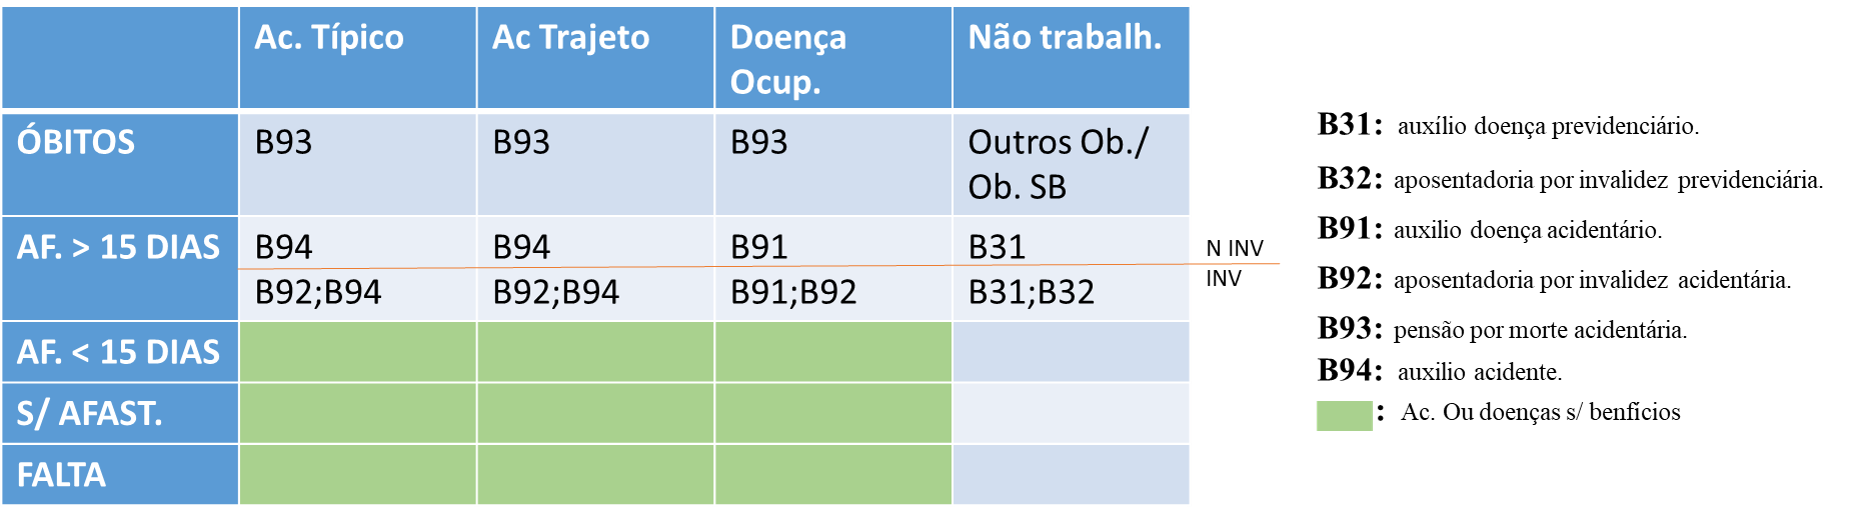
\includegraphics{../figures/quadro_beneficios.png}

\paragraph{B91 - Auxílio Doença Acidentário
(OK)}\label{b91---auxalio-doenaa-acidentario-ok}

Após o cálculo dos eventos serão calculados os benefícios gerados a
partir dos mesmos.

\[N_{b91} = Nev_{ocupacional, af>15}\]

\paragraph{B92 - Aposentadoria por Invalidez Acidentária
(OK)}\label{b92---aposentadoria-por-invalidez-acidentaria-ok}

O número de benefícios concedidos \(N_{b92}\) será igual ao número
de afastamentos menor do que quinze dias \(Nev_{af_{<15},k}\).

\[N_{b92} = \sum_{k=1}^{K92}{Nev_{af_{>15},k}}  * P_{inval} , onde \ K92 = \{típico \ , trajeto \  ou \ doença \ ocupacional\} \]
A probabilidade de invalidez P\_\{inval\} será igual para cada tipo de
acidente \(k\).

\paragraph{B93 - Pensão por Morte Acidentária
(OK)}\label{b93---pensao-por-morte-acidentaria-ok}

\[N_{b93} = \sum_{k=1}^{K93}Nev_{obito, k}, onde \ K93 = \{típico \ , trajeto \  ou \ doença \ ocupacional\}\]

\paragraph{B94 - Auxílio Acidente
(OK)}\label{b94---auxalio-acidente-ok}

\[N_{b94} = (Nev_{af>15},_{traj} + Nev_{af>15},_{tipico})\] Deve-se
notar que, para fins de FAP, os eventos não devem considerar os
acidentes de trajetos. Caso o número de benefícios separado por
espécie seja apenas relevante para o FAP, os acidentes de trajetos
devem ser removidos das fórmulas acima. Caso contrário, devem ser
criadas variáveis em separado para fins de FAP e para outros fins.

\paragraph{B31 - Auxílio Doença Previdenciário
(OK)}\label{b31---auxalio-doenaa-previdenciario-ok}

Os Auxílios por Doença Previdenciário serão calculados a partir dos
eventos não relacionados ao trabalho
\(Nev_{NRelacionadoAoTrabalho, af>15}\).
\[N_{b31} = Nev_{NRelacionadoAoTrabalho, af>15}\]

\paragraph{B32 - Aposentadoria Invalidez Previdenciário
(OK)}\label{b32---aposentadoria-invalidez-previdenciario-ok}

As aposentadorias por invalidez previdenciárias serão calculadas a
partir dos eventos não relacionados ao trabalho
\(Nev_{NRelacionadoAoTrabalho, af>15}\).
\[N_{b32} = Nev_{NRelacionadoAoTrabalho, af>15} * P_{Invalidez}\]

\paragraph{Número de benefícios acumulados
(OK)}\label{namero-de-benefacios-acumulados-ok}

O número de benefícios acumulado será calculado de acordo com o
número de benefícios concedido até o período \(t\) em questão e o
número de benefícios inicial.
\[NB_{i,t} = \sum_{t=1}^{t} N_i,t + N_i,inicial \ \forall \ i \  \in \ B\]

\subsubsection{Categorias de
Benefícios}\label{categorias-de-benefacios}

\paragraph{Despesas Evitáveis}\label{despesas-evitaveis}

\subparagraph{Despesas com Reclamatórias
Trabalhistas}\label{despesas-com-reclamatarias-trabalhistas}

Esta subcategoria compreende as despesas evitadas com reclamatórias
trabalhistas (objeto da ação relacionadas Ã~ doenças e acidentes do
trabalho) após a implementação integral da iniciativa.

\[{D}_{reclamatorias} = c_{medrec}*n_{reclamatorias} \]

Número de Reclamatórias Trabalhistas

O número de reclamatórias trabalhistas será calculado considerando o
número de funcionários desligados total multiplicado pela
probabilidade de ajuizar e ganhar uma reclamatória trabalhista cujo
objeto da ação está relacionado Ã~ saúde e Segurança do Trabalho.

\[n_{reclamatorias} = f_{desligacumulado} * p_{ajuizarEganharreclamatoria} \]

\subparagraph{Acidente / Doença Ocupacional -
Invalidez}\label{acidente-doenaa-ocupacional---invalidez}

Esta subcategoria compreende as despesas evitadas com incapacitação
parcial ou total provocada por acidente típico, doença ocupacional ou
acidente de trajeto após a implementação integral da iniciativa.

Possibilidade 1: Todos os custos incorridos nesta rúbrica entram para o
cálculo do FAP e não deveriam ser contados em duplicidade.

Possibilidade 2: Existem despesas que não estão em nenhuma outra
categoria e que deveriam ser contabilizados aqui. A princípio estamos
na possibilidade 1. A categoria será excluída caso a possibilidade 1
se confirme.

\subparagraph{Ações Regressivas INSS}\label{aaaes-regressivas-inss}

Esta subcategoria compreende as despesas evitadas com ações
regressivas do INSS após a implementação integral da iniciativa. A
Ação Regressiva representa o ressarcimento de pagamento de benefícios
acidentários do empregador ao INSS. Lei 8213/91, artigo 120 :A ação
regressiva é a penalização adicional relacionada ao B91 - B94.

As despesas com ações regressivas relacionadas ao INSS serão
calculadas considerando o número de benefícios acumulado, e a
probabilidade de incidência de uma ação regressiva, e a despesa
média relacionada a uma ação regressiva. Além disso, um cenário de
crise poderá modular esta função. O custo médio ponderado dos
benefícios acumulados será calculado de acordo com os mesmos custos
médios informados para fins de FAP. Assume-se que as despesas de
ressarcimento da empresa para com o INSS são as mesmas despesas que o
INSS teve com o indivíduo que originou a ação regressiva.

\[D_{ações regressivas INSS} =  \sum_{i=1}^{B} nacumulado_i * p_{acaoregress,} * (1+(f_{crise}*crise))  * \frac{\sum_{i=1}^{B} (nacumulado_i *cmed_{i})}{\sum_{i=1}^{B} nacumulado_i} \]

\subparagraph{Ausência para Tratamento}\label{ausancia-para-tratamento}

Esta subcategoria compreende as despesas evitadas com a ausência do
trabalhador afastado para tratamento após a implementação integral da
iniciativa. Os custos desta categoria já estão incluidos na categoria
de absenteísmo.

\subparagraph{Despesas Médicas}\label{despesas-madicas}

Esta subcategoria compreende as despesas evitadas com medicamento e
atendimento médico para tratamento dos acidentes de trabalho após a
implementação integral da iniciativa.

\[D_{medicas} = d_{medio} * (\sum_{k=1}^{K'} {\sum_{c=1}^{C'} {n_{acidentes \ k,c}}}) \ onde \  K' = \{{Típico},{Doença\ Ocupacional}\} \ e \ C' = \{{>15},<15,Sem\ Afast\}\]

\subparagraph{Reajustes do plano de Saúde
(OK)}\label{reajustes-do-plano-de-saade-ok}

Esta subcategoria compreende as despesas evitadas com planos de saúde
via alteração da taxa de sinistralidade após a implementação
integral da iniciativa. A despesa com o plano de saúde de cada período
será calculada de acordo com a despesa do ano anterior, acrescida de um
percentual de reajuste estimado.

\[D_{planosaude,t} = D_{planosaude,t-1} * (1 + Reaj_{estimado,t})\]

O reajuste estimado (parcela variável, excluindo variações
inflacionárias) será obtido por meio de uma regressão, comparada aos
índices de frequência e gravidade, considerando a soma de acidentes do
ano anterior. Deve-se observar que o intercepto \(B_0\) e o coeficiente
\(B_f\) e \(B_g\)serão estimados a priori, e aplicados pelo modelo a
cada ano. As ações regressivas relacionadas ao SUS contra o plano de
saúde entrarão indiretamente nesta regressão (presente nos índices).

\[Reaj_{estimado,t} = \beta_{0,reaj} +\beta_{f,reaj} * I_{fa} + \beta_{g,reaj} * I_{ga}\]

\subparagraph{Interrupção Operacional por
Acidente/Morte}\label{interrupaao-operacional-por-acidentemorte}

As despesas com interrupção operacional serão calculadas considerando
o número de acidentes típicos, o tempo de interrução (o qual pode
ser estimado pelo número total de dias de interrupção sobre o número
total de acidentes) e o lucro cessante médio diário oriúndo de cada
acidente.

Opção 1: Coletar os dias médios de interrupção geral.

Opção 2: Estimar os dias de interrupção de modo separado por tipo de
acidentes (ex.: Ã``bito, Afastamento maior que 15, menor que 15, ou sem
Afastamento.). Possívelmente, há como manter os dias de interrupção
por óbito em separado.

\[D_{interdicao,acidente} = n_{acidentestipico} * dias_{interr,acidente} * lucrocessante\]

\subparagraph{Interdições Por
Fiscalização}\label{interdiaaes-por-fiscalizaaao}

As despesas com interdições por fiscalização serão calculadas de
acordo com a probabilidade de interdição, o número médio de dias
relacionados Ã~ interdição por fiscalização e o lucro cessante
médio diário oriúndo de cada interdição. Adicionalmente, esta
equação pode ser modulada pela projeção de uma crise financeira. O
evento de interdição por fiscalização \(Evento_{interdicao}\) será
estimado com uma distribuição binomial.

Pergunta 1: Toda interdição gera uma multa?

Pergunta 2: Toda multa gera uma interdição?

Se 1= Sim e 2 = Não, então pode-se vincular os eventos de interdição
com multa, incluindo uma probabilidade de multa gerar interdição. Se 1
e 2 = Sim, então todos os eventos de multa gerarão interdição. Se 1
e 2 = Não, o formato atual deve ser mantido.

\[D_{interdicao, fiscalizacao} = Evento_{interdicao} * (1+(f_{crise}*crise)) * dias_{interr,fiscalizacao} * lucrocessante \]

\subparagraph{Reabilitação do Trabalhador
(OK)}\label{reabilitaaao-do-trabalhador-ok}

Trabalhadores passíveis de esforços de reabilitação incluem
trabalhadores préviamente afastados por mais do que 15 dias. O custo de
reabilitação contém todos os custos relacionados Ã~ reabilitação,
inclusive os custos de manutenção do reabilitado, inclusive para além
do período de simulação. Custos relacionados Ã~ iniciativas de
reabilitação de grupos de risco e PCDs serão considerados no modelo
por meio da redução do risco de eventos. Desta maneira, não serão
contabilizados como um benefício direto nesta categoria.

\[D_{reab} = custo_{reab} * \sum_{c=1}^{C}(Nev_{c, af>15} + Nev_{c, af<15}) * preab \]

\paragraph{Reduções Fiscais}\label{reduaaes-fiscais}

\subparagraph{Exposição Ã~ Multas}\label{exposiaao-a-multas}

As despesas oriúndas da exposição Ã~ multa serão calculadas
considerando-se o número de multas aplicadas e o custo médio da multa.
Adicionalmente, o número de multas também pode ser modulado pela
ocorrência de uma crise.

Opção 1: Considerar a Exposição á multas de modo geral.

Opção 2: Criar 5 slots de números de multas a considerar. (Com este
formato será possível segregar categorias de multa de acordo com a
empresa, ou, no limite, usar apenas um dos slots).

Opção 3: Estimar custos médios de multa, e probabilidades de multa de
modo individualizado (para cada NR).

\[D_{multas}= (1+(f_{crise}*crise)) * N_{multa_l}' * C_{med_l}\]

Número de multas

O número de múltas aplicado será calculado de acordo com o
atingimento da legislação (variável binária 0 ou 1) e o número de
multas estimado pela regressão.
\[N_{multa_l}' = (1 - Atendlegisl_l) * N_{multa_l}\]

O número de multas será estimado de acordo com os eventos de acidentes
típicos e doenças ocupacionais.
\[ N_{multa_l} =  \beta_{0,multa_l} + \beta_{1,multa_l} * (Nev_{tipico} + Nev_{doenocup})\]

\subparagraph{FAP (OK)}\label{fap-ok}

Fonte para o cálculo do FAP utilizada:
\url{http://sislex.previdencia.gov.br/paginas/72/MF-CNP/2017/1329.htm}

Índices de Frequência, Gravidade e Custo

Os óbitos sem benefício são exatamente isso: Ã``bitos acidentários
que não receberam benefício (por algum motivo).

\[I_f = \frac{(n_{obitossembeneficio}+n_{b92}+n_{b91}+n_{b93}+n_{b94})}{f} * 1000\]

Para fins de cálculo do FAP, o índice de frequência deve considerar
os dois últimos anos.

\[I_f,t = \frac{I_{f,t-1} + I_{f,t-2}}{2}\]

O índice de gravidade será calculado a partir desta fórmula:

\[I_g = \frac{(0.1*n_{b91}+0.3*n_{b92}+0.5*(n_{b93}+n_{obitossembeneficio})+0.1*n_{b94})}{f}* 1000\]

E o índice de custo será calculado a partir desta fórmula:

\[I_c = \frac{\sum_{i=91}^{94} n_{i}*cmed_{i}}{folhamédia} * 1000\]

Percentis

Percentis são calculados de acordo com os índices nos dois anos
anteriores.Os percentis dependem do posicionamento da empresa em
relação Ã~s demais. Específicamente a função \(Pos(I_{t})\) é
calculada pela previdência de acordo com os índices de todas as
empresas no mesmo subgrupo do CNAE da empresa em questão.

\[p_t = \frac{100*(Pos(I_{t})-1)}{n-1}\]

Considerando a necessidade de estimar o percentil a partir dos eventos,
será utilizada uma regressão linear relacionando o percentil ao
número de eventos observados na empresa. Considerando que o FAP é
calculado utilizando os últimos dois anos, a regressão também deve
considerar este mesmo período.

\[p_t = \beta_{0,percent} + \beta_{1,percent} *  +\beta_{t,percent} * I_t \ \forall t \in \{f,g,c\}\]

Índice Composto

O IC, por sua vez, é calculado de acordo com os percentis de gravidade
\(p_g\), frequência \(p_{f}\) e custo\(p_c\):

\[IC = (0,5*p_g + 0,35*p_{f}+0,15*p_c)0,02\]

Cálculo Final do FAP

Para o cálculo do FAP, o turnover da empresa deve ser calculado
considerando os ultimos dois anos. Deve ser observado o item 3.8, que
indica que " Serão consideradas no cálculo apenas as rescisões sem
justa causa, por iniciativa do empregador, inclusive rescisão
antecipada do contrato a termo; e as rescisões por término do contrato
a termo."

\[turnover_{FAP} = \frac{\frac{min(admissoes_{t-1}, recisoes{t-1})}{f_{t-1}} + \frac{min(admissoes_{t-2}, recisoes_{t-2})}{f_{t-2}}}{2}\]

Para fins de modelagem, o turnover FAP utilizará o cálculo do Turnover
geral mencionado anteriormente, ainda assim considerando a ponderação
de dois anos anteriores.
\[turnover_{FAP} = \frac{Turn_{geral,t-1} + Turn_{geral,t-2}}{2}\]

Ajuste 1 - Aplicado para os casos onde o IC \textless{} 1, de modo que o
FAP será no mínimo 0,5.
\[FAP = 0,5 + 0,5 * IC \ if \ (IC < 1, turnover_{FAP} < 0,75) \]

Ajuste 2 - aplicado para os casos onde a empresa obteve turnover maior
do que 0,75.

\[FAP = 1 \ if \ IC < 1, (turnover_{FAP} > 0,75)\]

Ajuste 3 - aplicado para os casos onde a empresa pode receber um
desconto (bônus) de 0,15 em seu FAP.

\[FAP = IC - (IC-1)*0,15 \ \ if \ (IC > 1, n_{b92,t-2}+n_{b93t-2} = 0)\]

Ajuste 4 - aplicado para o caso onde a empresa não pode obter o
desconto (bônus) de 0,15.

\[FAP = IC  \ if \ (IC > 1, n_{b92,t-2}+n_{b93t-2} > 0) \] Ajuste 5 - Se
a empresa tem menos do que dois anos, o FAP será igual a 1

\[FAP = 1  \ if \ (T_{idadeempresa} <= 2) \]

RAT Ajustado

O \(RAT\) varia entre 1 e 3, de acordo com o CNAE da empresa em
questão. \[RAT \in \{1,2,3\}\]

\[RAT_{ajust} = (FAP * RAT)\]

As despesas com seguro acidentário do trabalho \(D_{sat}\) serão
calculadas de acordo com as estimativas do \(FAP\) (\(0,005 - 0,02\)) e
\(RAT\) . Observar que o RAT ajustado calculado em um determinado ano
será usado no ano seguinte para o cálculo da despesa.

\[D_{sat} = RAT_{ajust,t-1}* F\] Exemplo: Período Base de cálculo:
2014 e 2015. Cálculo do FAP: 2016. Vigência: 2017.

\paragraph{Intangível}\label{intangavel}

\subparagraph{Imagem da Empresa}\label{imagem-da-empresa}

Os benefícios da inciativa relacionados Ã~ imagem foram desmembradas em
duas variáveis. Uma variável considera o ganho obtido com expansão de
receita, e uma segunda apresenta o ganho relacionado Ã~s despesas com
contratação.

\[D_{imagem}  = D_{imagem, contratacao} + D_{imagem, receita}\] 4
alternativas pensadas para estimar a variável \(D_{imagem, receita}\)
são estas:

\begin{enumerate}
\def\labelenumi{\Alph{enumi})}
\item
  Ganho de Mercado Informado;
\item
  Ganho de Mercado Informado apenas quando se atende a uma taxa máxima
  de frequência e gravidade (considerando as taxas do INSS);
\item
  Regressão considerando os índices do INSS e PIB, explicando a
  variação das propostas
  (\(Propostas * chance de conversão * Receita * margem média\));
\item
  Não fazer nada: Não inserir o ganho de receita via imagem no modelo.
\end{enumerate}

As despesas com imagem relacionadas a contratação serão estimadas
considerando o tempo de contratação médio, custo de contratação e
número médio de funcionários contratados.

\[D_{imagem, contratacao} =  (t_{contrat,t} - t_{contrat,t0}) * cmed_{diario} * Turn_geral * f\]

A variável de tempo de contratação será estimada por meio de uma
regressão linear, considerando o número de eventos do ano anterior
(considerando acidentes com afastamento maior do que 15 dias e óbitos).

\[t_{contrat} = \beta_{0,tcontrat} + \beta_{f,tcontrat} * I_{fa} + \beta_{g,tcontrat} * I_{ga} + \beta_{PIB,tcontrat} * var_{PIB}\]

\subparagraph{Engajamento e Clima organizacional
(OK)}\label{engajamento-e-clima-organizacional-ok}

As despesas relacionadas a engajamento e clima organizacional serão
calculadas a partir de desligamentos voluntários projetados.

\[D_{clima} = Deslig_{voluntarios} * c_{sub}\]

\[Deslig_{voluntarios} = Perc_{desligvoluntarios} * f \]

A variável de percentual de desligamento voluntário será calculada
por meio de uma regressão linear, considerando os eventos calculados.

\[Perc_{desligvoluntarios} = \beta_{0,desvolunt} +\beta_{f,desvolunt} * I_{fa} + \beta_{g,desvolunt} * I_{ga} + \beta_{PIB,desvolunt} * var_{PIB}\]

\paragraph{Melhor Uso dos Recursos}\label{melhor-uso-dos-recursos}

\subparagraph{Despesas com Turnover SST / FPS
(OK)}\label{despesas-com-turnover-sst-fps-ok}

As despesas com Turnover \(D_{tur}\) serão calculadas com base no
número de funcionários afastados por problemas relacionados Ã~ SST
\(n_{afast}\) e no custo médio de substituição dos
funcionários\(c_{sub}\).

\[D_{tur} = (Nev_{af_{>15},k} + Nev_{obito,k}) * c_{sub}\]

\subparagraph{Despesas com Absenteísmo
(OK)}\label{despesas-com-absenteasmo-ok}

As despesas com Absenteísmo \(D_{abs}\) serão calculadas com base no
número de dias de absenteísmo por problemas relacionados Ã~ SST
\(d_{abs}\), no número de horas trabalhadas por dia \(h\) e no custo em
mão de obra médio horário \(c_{mdo}\).

\[D_{abs} = d_{abs} * h * c_{mdo}\]

Dias de Absenteísmo

Os dias de absenteísmo levam em consideração os afastamentos menores
do que 15 dias \(Nev_{af<15,k}\) e as faltas.

\[ d_{abs} = Nev_{af<15,k} * D_{medioafast<15} + Nfalta\]

\subparagraph{Presenteísmo (OK)}\label{presenteasmo-ok}

Assim como o absenteísmo, o presenteísmo será calculado considerando
o custo médio da mão de obra, o número de horas trabalhadas e o
índice de presenteísmo. O índice será informado para a situação
com iniciativa e sem iniciativa. A decisão a ser tomada é como estimar
o percentual de presenteísmo (ou seja, se o percentual de presenteísmo
atual será informado diretamente ou estimado por meio de um instrumento
específico).

\[D_{presenteismo} = Perc_{present} * f * h * c_{mdo}\]

\subparagraph{Refugo e Retrabalho}\label{refugo-e-retrabalho}

As despesas com refugo e retrabalho serão calculadas considerando o
número de eventos típicos e doenças ocupacionais, e um custo médio
em refugo e retrabalho por evento.

\[D_{refug_retr} = cmed_{refretr} * Nev_{tipico,ocupac}\]

\subparagraph{MP, Insumos, Equipamentos
Operação}\label{mp-insumos-equipamentos-operaaao}

De modo similar, as despesas com matéria prima, insumos e equipamentos
serão calculadas considerando o número de eventos típicos e doenças
ocupacionais, e um custo médio por evento.

\[D_{MP,Ins,Eq} = cmed_{MP,Ins,Eq} * Nev_{tipico,ocupac}\]

\subparagraph{Qualidade}\label{qualidade}

Os ganhos em qualidade \(D_{qual,t}\) serão calculados considerando os
savings médios unitários em qualidade \(sav_{qual}\)projetados pela
iniciativa, multiplicados pela produção projetada do período.

Opção 1: Variação no Volume de Venda Projetada:
\[D_{qual,t} = var_{volumevenda,t} * margemmed_{unitario,t} * prod_{proj,t}\]

Opção 2: Regressão a partir dos custos e índices de frequência e
gravidade:
\[D_{qual,t} = var_{volumevenda,t} * margemmed_{unitario,t} * prod_{proj,t}\]

\[var_{volumevenda,t} = \beta_{0,volumevenda} +\beta_{f,volumevenda} * I_{fa} + \beta_{g,volumevenda} * I_{ga} + \beta_{PIB,volumevenda} * var_{PIB}\]

\subparagraph{Produtividade}\label{produtividade}

Os ganhos em produtividade \(D_{prod,t}\) serão calculados considerando
os savings médios unitários em mão-de-obra \(sav_{MDO}\)projetados
pela iniciativa, multiplicados pela produção projetada do período.

Opção 1: Saving unitário informado da inciativa
\[D_{prod,t} = sav_{MDO} * prod_{proj,t}\]

Opção 2: Regressão a partir dos custos e índices de frequência e
gravidade: O custo médio unitário será igual ao total produzido e os
custo operacional.

\[D_{prod,t} = varcustomed_{unitario,t} * customed_{unitario,t} * prod_{proj,t}\]

\[varcustomed_{unitario,t} = \beta_{0,customed} +\beta_{f,customed} * I_{fa} + \beta_{g,customed} * I_{ga} + \beta_{PIB,customed} * var_{PIB}\]

\subsection{Lista de Símbolos e
Definições}\label{lista-de-sambolos-e-definiaaes}

\begin{longtable}[]{@{}ll@{}}
\toprule
\begin{minipage}[b]{0.07\columnwidth}\raggedright\strut
\textbf{Símbolo}\strut
\end{minipage} & \begin{minipage}[b]{0.87\columnwidth}\raggedright\strut
\textbf{Definição}\strut
\end{minipage}\tabularnewline
\midrule
\endhead
\begin{minipage}[t]{0.07\columnwidth}\raggedright\strut
\(\theta\)\strut
\end{minipage} & \begin{minipage}[t]{0.87\columnwidth}\raggedright\strut
Taxa de desconto a utilizar para trazer o valor dos custos e benefícios
a valor presente.\strut
\end{minipage}\tabularnewline
\begin{minipage}[t]{0.07\columnwidth}\raggedright\strut
\(Atendlegisl_{l}\)\strut
\end{minipage} & \begin{minipage}[t]{0.87\columnwidth}\raggedright\strut
Atendimento da legislação\strut
\end{minipage}\tabularnewline
\begin{minipage}[t]{0.07\columnwidth}\raggedright\strut
\(B_{i}\)\strut
\end{minipage} & \begin{minipage}[t]{0.87\columnwidth}\raggedright\strut
Benefício atribuído ao conjunto de iniciativas em questão em valor
presente, onde \(i\) indexa a categoria de Iniciativa.\strut
\end{minipage}\tabularnewline
\begin{minipage}[t]{0.07\columnwidth}\raggedright\strut
\(B_i\)\strut
\end{minipage} & \begin{minipage}[t]{0.87\columnwidth}\raggedright\strut
Benefício gerado pela iniciativa (ou iniciativas) avaliadas, na
categoria \(i\), em unidades monetárias.\strut
\end{minipage}\tabularnewline
\begin{minipage}[t]{0.07\columnwidth}\raggedright\strut
\(c\)\strut
\end{minipage} & \begin{minipage}[t]{0.87\columnwidth}\raggedright\strut
Índice que indexa os tipos de eventos.\strut
\end{minipage}\tabularnewline
\begin{minipage}[t]{0.07\columnwidth}\raggedright\strut
\(c_{mdo}\)\strut
\end{minipage} & \begin{minipage}[t]{0.87\columnwidth}\raggedright\strut
Custo médio horário da mão de obra.\strut
\end{minipage}\tabularnewline
\begin{minipage}[t]{0.07\columnwidth}\raggedright\strut
\(c_{medrec}\)\strut
\end{minipage} & \begin{minipage}[t]{0.87\columnwidth}\raggedright\strut
Custo Médio da Reclamatória.\strut
\end{minipage}\tabularnewline
\begin{minipage}[t]{0.07\columnwidth}\raggedright\strut
\(c_{sub}\)\strut
\end{minipage} & \begin{minipage}[t]{0.87\columnwidth}\raggedright\strut
Custo de substituição de um funcionário.\strut
\end{minipage}\tabularnewline
\begin{minipage}[t]{0.07\columnwidth}\raggedright\strut
\(C_i\)\strut
\end{minipage} & \begin{minipage}[t]{0.87\columnwidth}\raggedright\strut
Custo atribuído ao conjunto de inciativas em questão, onde \(j\)
indexa a categoria de custos.\strut
\end{minipage}\tabularnewline
\begin{minipage}[t]{0.07\columnwidth}\raggedright\strut
\(cmed_{contratacao}\)\strut
\end{minipage} & \begin{minipage}[t]{0.87\columnwidth}\raggedright\strut
Custo médio de contratação de um funcionário.\strut
\end{minipage}\tabularnewline
\begin{minipage}[t]{0.07\columnwidth}\raggedright\strut
\(cmed_{MP, Ins, Eq}\)\strut
\end{minipage} & \begin{minipage}[t]{0.87\columnwidth}\raggedright\strut
Custo médio com matéria prima, insumos e equipamentos por
evento.\strut
\end{minipage}\tabularnewline
\begin{minipage}[t]{0.07\columnwidth}\raggedright\strut
\(cmed_{refretr}\)\strut
\end{minipage} & \begin{minipage}[t]{0.87\columnwidth}\raggedright\strut
Custo médio em refugo e retrabalho por evento.\strut
\end{minipage}\tabularnewline
\begin{minipage}[t]{0.07\columnwidth}\raggedright\strut
\(Cmedmulta_{l}\)\strut
\end{minipage} & \begin{minipage}[t]{0.87\columnwidth}\raggedright\strut
Custo médio da multa originada pela lei \(l\)\strut
\end{minipage}\tabularnewline
\begin{minipage}[t]{0.07\columnwidth}\raggedright\strut
\(cmedregressiva_{i}\)\strut
\end{minipage} & \begin{minipage}[t]{0.87\columnwidth}\raggedright\strut
Custo médio de uma ação regressiva do tipo \(i\).\strut
\end{minipage}\tabularnewline
\begin{minipage}[t]{0.07\columnwidth}\raggedright\strut
\(crise\)\strut
\end{minipage} & \begin{minipage}[t]{0.87\columnwidth}\raggedright\strut
Variável que indica a projeção de uma crise no ano em questão.\strut
\end{minipage}\tabularnewline
\begin{minipage}[t]{0.07\columnwidth}\raggedright\strut
\(custo_{reab}\)\strut
\end{minipage} & \begin{minipage}[t]{0.87\columnwidth}\raggedright\strut
Custos médio com a reabilitação do trabalhador.\strut
\end{minipage}\tabularnewline
\begin{minipage}[t]{0.07\columnwidth}\raggedright\strut
\(customed_{unitario, t}\)\strut
\end{minipage} & \begin{minipage}[t]{0.87\columnwidth}\raggedright\strut
Custo médio unitário de produção no período \(t\).\strut
\end{minipage}\tabularnewline
\begin{minipage}[t]{0.07\columnwidth}\raggedright\strut
\(D\)\_\{medicas\}\strut
\end{minipage} & \begin{minipage}[t]{0.87\columnwidth}\raggedright\strut
Despesas evitadas com medicamento e atendimento médico para tratamento
dos acidentes de trabalho.\strut
\end{minipage}\tabularnewline
\begin{minipage}[t]{0.07\columnwidth}\raggedright\strut
\(d_{abs}\)\strut
\end{minipage} & \begin{minipage}[t]{0.87\columnwidth}\raggedright\strut
Número de dias de absenteísmo por problemas relacionados Ã~ SST e
FPS.\strut
\end{minipage}\tabularnewline
\begin{minipage}[t]{0.07\columnwidth}\raggedright\strut
\(D_{ações regressivas INSS}\)\strut
\end{minipage} & \begin{minipage}[t]{0.87\columnwidth}\raggedright\strut
Despesas relacionadas a Ações Regressivas.\strut
\end{minipage}\tabularnewline
\begin{minipage}[t]{0.07\columnwidth}\raggedright\strut
\(D_{clima}\)\strut
\end{minipage} & \begin{minipage}[t]{0.87\columnwidth}\raggedright\strut
Despesas relacionadas a clima organizacional.\strut
\end{minipage}\tabularnewline
\begin{minipage}[t]{0.07\columnwidth}\raggedright\strut
\(D_{i, asis}\)\strut
\end{minipage} & \begin{minipage}[t]{0.87\columnwidth}\raggedright\strut
Despesa ocorrida na categoria \(i\), considerando o cenário as
is.\strut
\end{minipage}\tabularnewline
\begin{minipage}[t]{0.07\columnwidth}\raggedright\strut
\(D_{i, inic}\)\strut
\end{minipage} & \begin{minipage}[t]{0.87\columnwidth}\raggedright\strut
Despesa ocorrida na categoria \(i\), considerando a realização da
iniciativa.\strut
\end{minipage}\tabularnewline
\begin{minipage}[t]{0.07\columnwidth}\raggedright\strut
\(D_{medioafast<15}\)\strut
\end{minipage} & \begin{minipage}[t]{0.87\columnwidth}\raggedright\strut
Dias médios de afastamento menores que 15 dias.\strut
\end{minipage}\tabularnewline
\begin{minipage}[t]{0.07\columnwidth}\raggedright\strut
\(D_{MP,Ins,Eq}\)\strut
\end{minipage} & \begin{minipage}[t]{0.87\columnwidth}\raggedright\strut
Despesas com matéria prima, insumos e equipamentos.\strut
\end{minipage}\tabularnewline
\begin{minipage}[t]{0.07\columnwidth}\raggedright\strut
\(D_{multas}\)\strut
\end{minipage} & \begin{minipage}[t]{0.87\columnwidth}\raggedright\strut
Despesas oriundas por exposição Ã~ multas.\strut
\end{minipage}\tabularnewline
\begin{minipage}[t]{0.07\columnwidth}\raggedright\strut
\(D_{planosaude, t-1}\)\strut
\end{minipage} & \begin{minipage}[t]{0.87\columnwidth}\raggedright\strut
Despesas com o plano de saúde do período anterior.\strut
\end{minipage}\tabularnewline
\begin{minipage}[t]{0.07\columnwidth}\raggedright\strut
\(D_{planosaude,t}\)\strut
\end{minipage} & \begin{minipage}[t]{0.87\columnwidth}\raggedright\strut
Despesas evitadas com planos de saúde via alteração da taxa de
sinistralidade.\strut
\end{minipage}\tabularnewline
\begin{minipage}[t]{0.07\columnwidth}\raggedright\strut
\(D_{prod, t}\)\strut
\end{minipage} & \begin{minipage}[t]{0.87\columnwidth}\raggedright\strut
Ganhos obtidos pela elevação da produtividade da mão-de-obra devido
ao ambiente seguro e saudável.\strut
\end{minipage}\tabularnewline
\begin{minipage}[t]{0.07\columnwidth}\raggedright\strut
\(D_{qual, t}\)\strut
\end{minipage} & \begin{minipage}[t]{0.87\columnwidth}\raggedright\strut
Ganhos obtidos com elevação da qualidade dos produtos e serviços
devido a melhora do ambiente seguro e saudável.\strut
\end{minipage}\tabularnewline
\begin{minipage}[t]{0.07\columnwidth}\raggedright\strut
\(D_{reclamatorias}\)\strut
\end{minipage} & \begin{minipage}[t]{0.87\columnwidth}\raggedright\strut
Despesas evitadas com reclamatórias trabalhistas.\strut
\end{minipage}\tabularnewline
\begin{minipage}[t]{0.07\columnwidth}\raggedright\strut
\(D_{refugretr}\)\strut
\end{minipage} & \begin{minipage}[t]{0.87\columnwidth}\raggedright\strut
Despesas com refugo e retrabalho.\strut
\end{minipage}\tabularnewline
\begin{minipage}[t]{0.07\columnwidth}\raggedright\strut
\(Dabs\)\strut
\end{minipage} & \begin{minipage}[t]{0.87\columnwidth}\raggedright\strut
Despesas com absenteísmo.\strut
\end{minipage}\tabularnewline
\begin{minipage}[t]{0.07\columnwidth}\raggedright\strut
\(Deslig_{voluntarios}\)\strut
\end{minipage} & \begin{minipage}[t]{0.87\columnwidth}\raggedright\strut
Funcionários desligados de forma voluntária.\strut
\end{minipage}\tabularnewline
\begin{minipage}[t]{0.07\columnwidth}\raggedright\strut
\(dias_{interr, evento}\)\strut
\end{minipage} & \begin{minipage}[t]{0.87\columnwidth}\raggedright\strut
Dias médios interruptidos por eventos.\strut
\end{minipage}\tabularnewline
\begin{minipage}[t]{0.07\columnwidth}\raggedright\strut
\(dias_{interr, fiscalizacao}\)\strut
\end{minipage} & \begin{minipage}[t]{0.87\columnwidth}\raggedright\strut
Dias médios interruptidos por fiscalização.\strut
\end{minipage}\tabularnewline
\begin{minipage}[t]{0.07\columnwidth}\raggedright\strut
\(Dimagem\)\strut
\end{minipage} & \begin{minipage}[t]{0.87\columnwidth}\raggedright\strut
Despesa total relacionada Ã~ imagem da empresa.\strut
\end{minipage}\tabularnewline
\begin{minipage}[t]{0.07\columnwidth}\raggedright\strut
\(Dimagem, contratacao\)\strut
\end{minipage} & \begin{minipage}[t]{0.87\columnwidth}\raggedright\strut
Despesa relacionada Ã~ imagem da empresa, ocorrida em função do
aumento de tempo de contratação em função de eventos
acidentários.\strut
\end{minipage}\tabularnewline
\begin{minipage}[t]{0.07\columnwidth}\raggedright\strut
\(Dimagem, receita\)\strut
\end{minipage} & \begin{minipage}[t]{0.87\columnwidth}\raggedright\strut
Ganho relacionado Ã~ imagem da empresa, obtido em função de aumento de
receita.\strut
\end{minipage}\tabularnewline
\begin{minipage}[t]{0.07\columnwidth}\raggedright\strut
\(Dinterdicao_{evento}\)\strut
\end{minipage} & \begin{minipage}[t]{0.87\columnwidth}\raggedright\strut
Despesas evitadas com interrupção operacional originados por acidentes
ou óbitos.\strut
\end{minipage}\tabularnewline
\begin{minipage}[t]{0.07\columnwidth}\raggedright\strut
\(Dinterdicao_{fiscalizacao}\)\strut
\end{minipage} & \begin{minipage}[t]{0.87\columnwidth}\raggedright\strut
Despesas evitadas com interdições por fiscalização.\strut
\end{minipage}\tabularnewline
\begin{minipage}[t]{0.07\columnwidth}\raggedright\strut
\(Dmed_{medicas}\)\strut
\end{minipage} & \begin{minipage}[t]{0.87\columnwidth}\raggedright\strut
Despesa médica média com medicamento e atendimento médico.\strut
\end{minipage}\tabularnewline
\begin{minipage}[t]{0.07\columnwidth}\raggedright\strut
\(Dpresenteismo\)\strut
\end{minipage} & \begin{minipage}[t]{0.87\columnwidth}\raggedright\strut
Despesas com presenteísmo.\strut
\end{minipage}\tabularnewline
\begin{minipage}[t]{0.07\columnwidth}\raggedright\strut
\(Dreab\)\strut
\end{minipage} & \begin{minipage}[t]{0.87\columnwidth}\raggedright\strut
Despesas com reabilitação do trabalhador.\strut
\end{minipage}\tabularnewline
\begin{minipage}[t]{0.07\columnwidth}\raggedright\strut
\(Dtur\)\strut
\end{minipage} & \begin{minipage}[t]{0.87\columnwidth}\raggedright\strut
Despesas com turnover.\strut
\end{minipage}\tabularnewline
\begin{minipage}[t]{0.07\columnwidth}\raggedright\strut
\(Evento_{fiscalizacao}\)\strut
\end{minipage} & \begin{minipage}[t]{0.87\columnwidth}\raggedright\strut
Probabilidade de acontecer um evento de interdização por
fiscalização.\strut
\end{minipage}\tabularnewline
\begin{minipage}[t]{0.07\columnwidth}\raggedright\strut
\(f\)\strut
\end{minipage} & \begin{minipage}[t]{0.87\columnwidth}\raggedright\strut
Número de Funcionários da Empresa.\strut
\end{minipage}\tabularnewline
\begin{minipage}[t]{0.07\columnwidth}\raggedright\strut
\(f_{crise}\)\strut
\end{minipage} & \begin{minipage}[t]{0.87\columnwidth}\raggedright\strut
Fator multiplicativo relacionado Ã~ ocorrência de uma crise
financeira.\strut
\end{minipage}\tabularnewline
\begin{minipage}[t]{0.07\columnwidth}\raggedright\strut
\(f_{desligacumulado}\)\strut
\end{minipage} & \begin{minipage}[t]{0.87\columnwidth}\raggedright\strut
Número de Funcionários desligados pela empresa.\strut
\end{minipage}\tabularnewline
\begin{minipage}[t]{0.07\columnwidth}\raggedright\strut
\(IC\)\strut
\end{minipage} & \begin{minipage}[t]{0.87\columnwidth}\raggedright\strut
Índice composto do FAP.\strut
\end{minipage}\tabularnewline
\begin{minipage}[t]{0.07\columnwidth}\raggedright\strut
\(Ic\)\strut
\end{minipage} & \begin{minipage}[t]{0.87\columnwidth}\raggedright\strut
Índice de custo do FAP.\strut
\end{minipage}\tabularnewline
\begin{minipage}[t]{0.07\columnwidth}\raggedright\strut
\(If\)\strut
\end{minipage} & \begin{minipage}[t]{0.87\columnwidth}\raggedright\strut
Índice de frequência do FAP.\strut
\end{minipage}\tabularnewline
\begin{minipage}[t]{0.07\columnwidth}\raggedright\strut
\(Ig\)\strut
\end{minipage} & \begin{minipage}[t]{0.87\columnwidth}\raggedright\strut
Índice de gravidade do FAP.\strut
\end{minipage}\tabularnewline
\begin{minipage}[t]{0.07\columnwidth}\raggedright\strut
\(k\)\strut
\end{minipage} & \begin{minipage}[t]{0.87\columnwidth}\raggedright\strut
Índice que indexa os tipos de acidentes.\strut
\end{minipage}\tabularnewline
\begin{minipage}[t]{0.07\columnwidth}\raggedright\strut
\(lucrocessante\)\strut
\end{minipage} & \begin{minipage}[t]{0.87\columnwidth}\raggedright\strut
Lucro cessante médio diário oriundo de cada acidente.\strut
\end{minipage}\tabularnewline
\begin{minipage}[t]{0.07\columnwidth}\raggedright\strut
\(margemmed_{unitario, t}\)\strut
\end{minipage} & \begin{minipage}[t]{0.87\columnwidth}\raggedright\strut
Margem média de contribuição unitária no período \(t\).\strut
\end{minipage}\tabularnewline
\begin{minipage}[t]{0.07\columnwidth}\raggedright\strut
\(N_{b31}\)\strut
\end{minipage} & \begin{minipage}[t]{0.87\columnwidth}\raggedright\strut
Número de Auxílios Doença Previdenciário.\strut
\end{minipage}\tabularnewline
\begin{minipage}[t]{0.07\columnwidth}\raggedright\strut
\(N_{b32}\)\strut
\end{minipage} & \begin{minipage}[t]{0.87\columnwidth}\raggedright\strut
Número de Aposentadorias Invalidez Previdenciário.\strut
\end{minipage}\tabularnewline
\begin{minipage}[t]{0.07\columnwidth}\raggedright\strut
\(N_{b91}\)\strut
\end{minipage} & \begin{minipage}[t]{0.87\columnwidth}\raggedright\strut
Número de Auxílios Doença Acidentário.\strut
\end{minipage}\tabularnewline
\begin{minipage}[t]{0.07\columnwidth}\raggedright\strut
\(N_{b92}\)\strut
\end{minipage} & \begin{minipage}[t]{0.87\columnwidth}\raggedright\strut
Número de Aposentadorias por Invalidez Acidentária.\strut
\end{minipage}\tabularnewline
\begin{minipage}[t]{0.07\columnwidth}\raggedright\strut
\(N_{b93}\)\strut
\end{minipage} & \begin{minipage}[t]{0.87\columnwidth}\raggedright\strut
Número de Pensões por Morte Acidentária.\strut
\end{minipage}\tabularnewline
\begin{minipage}[t]{0.07\columnwidth}\raggedright\strut
\(N_{b94}\)\strut
\end{minipage} & \begin{minipage}[t]{0.87\columnwidth}\raggedright\strut
Número de Auxílio Acidente.\strut
\end{minipage}\tabularnewline
\begin{minipage}[t]{0.07\columnwidth}\raggedright\strut
\(n_{reclamatorias}\)\strut
\end{minipage} & \begin{minipage}[t]{0.87\columnwidth}\raggedright\strut
Número de Reclamatórias trabalhistas relacionadas a SST.\strut
\end{minipage}\tabularnewline
\begin{minipage}[t]{0.07\columnwidth}\raggedright\strut
\(Nacumulado_{i}\)\strut
\end{minipage} & \begin{minipage}[t]{0.87\columnwidth}\raggedright\strut
Número de benefícios acumulados do tipo \(i\ \forall\ B\)\strut
\end{minipage}\tabularnewline
\begin{minipage}[t]{0.07\columnwidth}\raggedright\strut
\(NB_{i,t}\)\strut
\end{minipage} & \begin{minipage}[t]{0.87\columnwidth}\raggedright\strut
Número de benefícios acumulados, considerando o período atual e os
períodos anteriores. \(i\) indexa os tipos de benefícios,
\(i \in \ I =\{N_{b91}, N_{b92}, N_{b93}, N_{b94}\}\).\strut
\end{minipage}\tabularnewline
\begin{minipage}[t]{0.07\columnwidth}\raggedright\strut
\(Nev_{c,k}\)\strut
\end{minipage} & \begin{minipage}[t]{0.87\columnwidth}\raggedright\strut
Número de Eventos \(c\) gerados a partir do acidente do tipo
\(k\).\strut
\end{minipage}\tabularnewline
\begin{minipage}[t]{0.07\columnwidth}\raggedright\strut
\(Nfalta\)\strut
\end{minipage} & \begin{minipage}[t]{0.87\columnwidth}\raggedright\strut
Número total de faltas.\strut
\end{minipage}\tabularnewline
\begin{minipage}[t]{0.07\columnwidth}\raggedright\strut
\(Nmultas'_{l}\)\strut
\end{minipage} & \begin{minipage}[t]{0.87\columnwidth}\raggedright\strut
Número de multas aplicadas oriundas da lei \(l\).\strut
\end{minipage}\tabularnewline
\begin{minipage}[t]{0.07\columnwidth}\raggedright\strut
\(Nmultas_{l}\)\strut
\end{minipage} & \begin{minipage}[t]{0.87\columnwidth}\raggedright\strut
Número de multas estimados de acordo com os eventos de acidentes
típicos e doenças ocupacionais.\strut
\end{minipage}\tabularnewline
\begin{minipage}[t]{0.07\columnwidth}\raggedright\strut
\(p_{ajuizarEganharreclamatoria}\)\strut
\end{minipage} & \begin{minipage}[t]{0.87\columnwidth}\raggedright\strut
Probabilidade de um funcionário demitido entrar com uma reclamatória e
ganhar a causa.\strut
\end{minipage}\tabularnewline
\begin{minipage}[t]{0.07\columnwidth}\raggedright\strut
\(P_{Invalidez}\)\strut
\end{minipage} & \begin{minipage}[t]{0.87\columnwidth}\raggedright\strut
Percentual dos Acidentes com afastamento maior do que quinze dias que
gera invalidez.\strut
\end{minipage}\tabularnewline
\begin{minipage}[t]{0.07\columnwidth}\raggedright\strut
\(p_{reab}\)\strut
\end{minipage} & \begin{minipage}[t]{0.87\columnwidth}\raggedright\strut
a.\strut
\end{minipage}\tabularnewline
\begin{minipage}[t]{0.07\columnwidth}\raggedright\strut
\(p_{t}\)\strut
\end{minipage} & \begin{minipage}[t]{0.87\columnwidth}\raggedright\strut
Percentil de acorodo com o posicionamento da empresa em relação as
demais, onde \(t \in {f,g,c}\)\strut
\end{minipage}\tabularnewline
\begin{minipage}[t]{0.07\columnwidth}\raggedright\strut
\(p_iacaoregressiva\)\strut
\end{minipage} & \begin{minipage}[t]{0.87\columnwidth}\raggedright\strut
Probabilidade de acontecer uma ação regressiva.\strut
\end{minipage}\tabularnewline
\begin{minipage}[t]{0.07\columnwidth}\raggedright\strut
\(Perc_{desligvoluntarios}\)\strut
\end{minipage} & \begin{minipage}[t]{0.87\columnwidth}\raggedright\strut
Percentual de desligamento voluntário.\strut
\end{minipage}\tabularnewline
\begin{minipage}[t]{0.07\columnwidth}\raggedright\strut
\(Perc_{present}\)\strut
\end{minipage} & \begin{minipage}[t]{0.87\columnwidth}\raggedright\strut
Percentual de presenteísmo.\strut
\end{minipage}\tabularnewline
\begin{minipage}[t]{0.07\columnwidth}\raggedright\strut
\(Pev_{c}\)\strut
\end{minipage} & \begin{minipage}[t]{0.87\columnwidth}\raggedright\strut
Probabilidade do evento \(c\) ocorrer.\strut
\end{minipage}\tabularnewline
\begin{minipage}[t]{0.07\columnwidth}\raggedright\strut
\(Pev_{k}\)\strut
\end{minipage} & \begin{minipage}[t]{0.87\columnwidth}\raggedright\strut
Percentual de Funcionários que irá sofrer o evento \(k\) em um
período. Equivalente ao percentual de funcionários da empresa a sofrer
o evento.\strut
\end{minipage}\tabularnewline
\begin{minipage}[t]{0.07\columnwidth}\raggedright\strut
\(Pev_{k}\)\strut
\end{minipage} & \begin{minipage}[t]{0.87\columnwidth}\raggedright\strut
Probabilidade do tipo de acidente \(k\) ocorrer. Equivalente ao
percentual de funcionários da empresa a sofrer o evento.\strut
\end{minipage}\tabularnewline
\begin{minipage}[t]{0.07\columnwidth}\raggedright\strut
\(prod_{proj, t}\)\strut
\end{minipage} & \begin{minipage}[t]{0.87\columnwidth}\raggedright\strut
Produção projetada no período \(t\).\strut
\end{minipage}\tabularnewline
\begin{minipage}[t]{0.07\columnwidth}\raggedright\strut
\(prod_{proj, t}\)\strut
\end{minipage} & \begin{minipage}[t]{0.87\columnwidth}\raggedright\strut
Volume de produção projetada no período \(t\).\strut
\end{minipage}\tabularnewline
\begin{minipage}[t]{0.07\columnwidth}\raggedright\strut
\(RBC\)\strut
\end{minipage} & \begin{minipage}[t]{0.87\columnwidth}\raggedright\strut
Razão Benefício-Custo. Para 1 Real investido na iniciativa indicada,
retornam \(\alpha\) reais.\strut
\end{minipage}\tabularnewline
\begin{minipage}[t]{0.07\columnwidth}\raggedright\strut
\(Reaj_{estimado, t}\)\strut
\end{minipage} & \begin{minipage}[t]{0.87\columnwidth}\raggedright\strut
Percentual de reajuste estimado no período \(t\).\strut
\end{minipage}\tabularnewline
\begin{minipage}[t]{0.07\columnwidth}\raggedright\strut
\(t_{contrat}\)\strut
\end{minipage} & \begin{minipage}[t]{0.87\columnwidth}\raggedright\strut
Tempo de contratação médio de um funcionário.\strut
\end{minipage}\tabularnewline
\begin{minipage}[t]{0.07\columnwidth}\raggedright\strut
\(T_falta\)\strut
\end{minipage} & \begin{minipage}[t]{0.87\columnwidth}\raggedright\strut
Taxa de Faltas. (Faltas por Funcionário por Período).\strut
\end{minipage}\tabularnewline
\begin{minipage}[t]{0.07\columnwidth}\raggedright\strut
\(var_{volumevenda, t}\)\strut
\end{minipage} & \begin{minipage}[t]{0.87\columnwidth}\raggedright\strut
Variação no volume de venda projetada no período \(t\).\strut
\end{minipage}\tabularnewline
\begin{minipage}[t]{0.07\columnwidth}\raggedright\strut
\(varcustomed_{unitario, t}\)\strut
\end{minipage} & \begin{minipage}[t]{0.87\columnwidth}\raggedright\strut
Variação no custo médio unitário de produção.\strut
\end{minipage}\tabularnewline
\bottomrule
\end{longtable}


\end{document}
